\section*{Attachments}
    % \begin{equation}
    %     distancia = \sqrt{ (x_{goal} - x_{state})^2 + (y_{goal} - y_{state})^2 }
    %     \label{eq:distancia-dois-pontos}
    % \end{equation}
    
    % \begin{figure}[h!]
    %     \centering
    %     \includegraphics[width=0.5\hsize]{figuras/cnn.png}
    %     \caption{Estrutura da Rede Convolucional.}
    %     \label{fig:cnn-arq}
    % \end{figure}
    
    \begin{figure}[h]
        \centering
        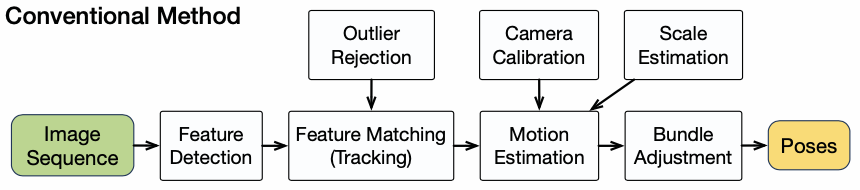
\includegraphics[width=0.75\columnwidth]{figuras/figura1.png}
        \caption{Classical pipeline for Visual Odometry.}
        \label{fig:1}
    \end{figure}

    \begin{figure}[h]
        \centering
        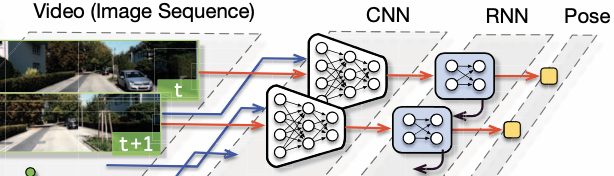
\includegraphics[width=0.75\columnwidth]{figuras/figura2.png}
        \caption{DeepVO pipeline for Visual Odometry.}
        \label{fig:2}
    \end{figure}
    
    \begin{figure}[h]
        \centering
        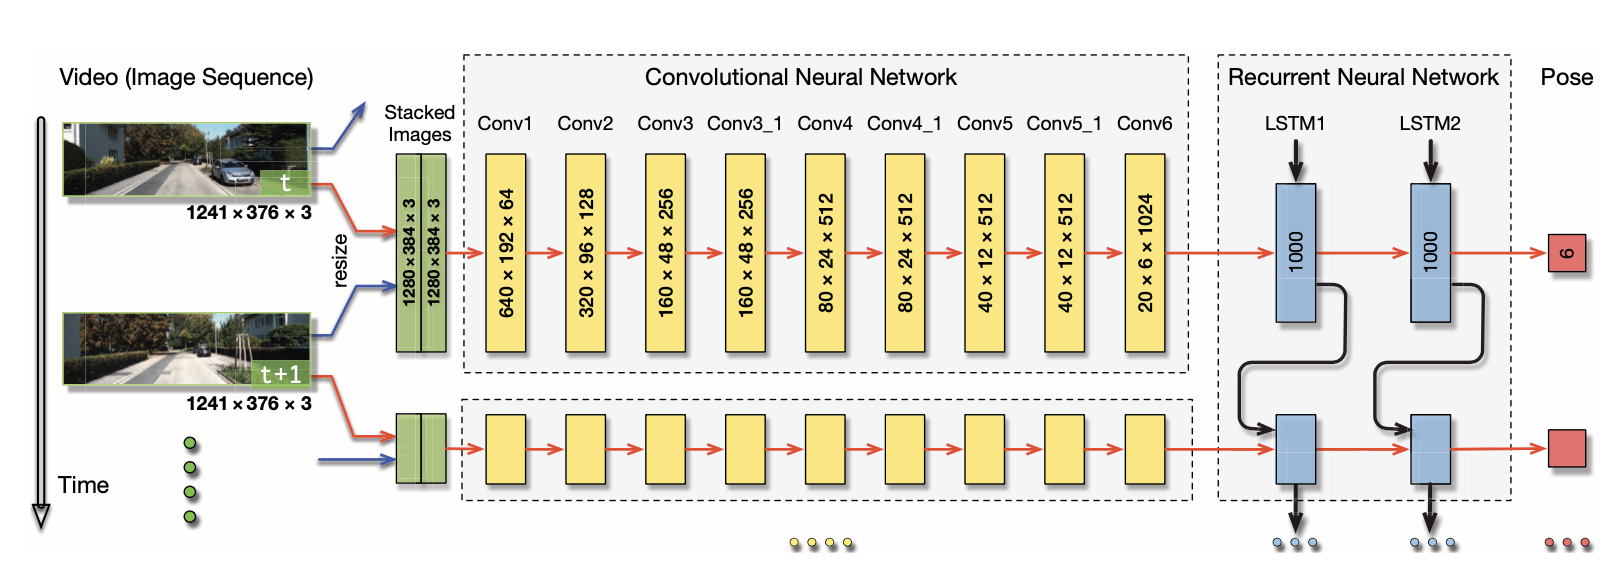
\includegraphics[width=0.65\columnwidth]{figuras/figura8.png}
        \caption{Architecture of the RCNN monocular VO system.}
        \label{fig:8}
    \end{figure}        
    
    \begin{figure}[h]
        \centering
        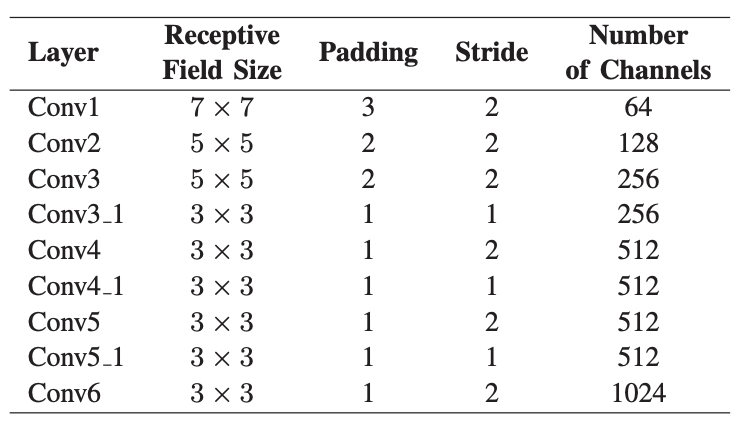
\includegraphics[width=0.65\columnwidth]{figuras/figura9.png}
        \caption{Configuration of the CNN for monocular VO system.}
        \label{fig:9}
    \end{figure}
    
    \begin{figure}[h]
        \centering
        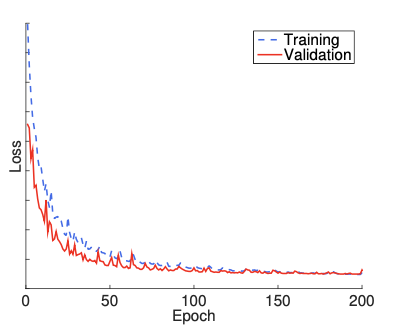
\includegraphics[width=0.65\columnwidth]{figuras/figura10.png}
        \caption{Training losses for the monocular VO system for the Wang paper.}
        \label{fig:10}
    \end{figure}
    
    \begin{figure}[h]
        \centering
        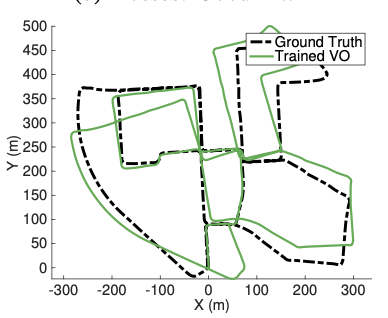
\includegraphics[width=0.65\columnwidth]{figuras/figura11.png}
        \caption{Obtained map for the monocular VO system under the training dataset for the Wang paper.}
        \label{fig:11}
    \end{figure}        

    \begin{figure}[h]
        \centering
        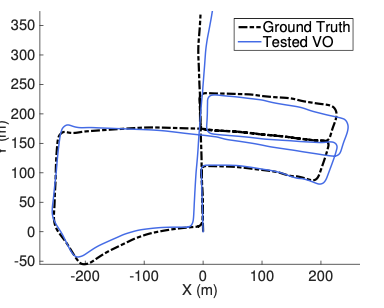
\includegraphics[width=0.65\columnwidth]{figuras/figura12.png}
        \caption{Obtained map for the monocular VO system under the test dataset for the Wang paper.}
        \label{fig:12}
    \end{figure}

    \begin{figure}[h]
        \centering
        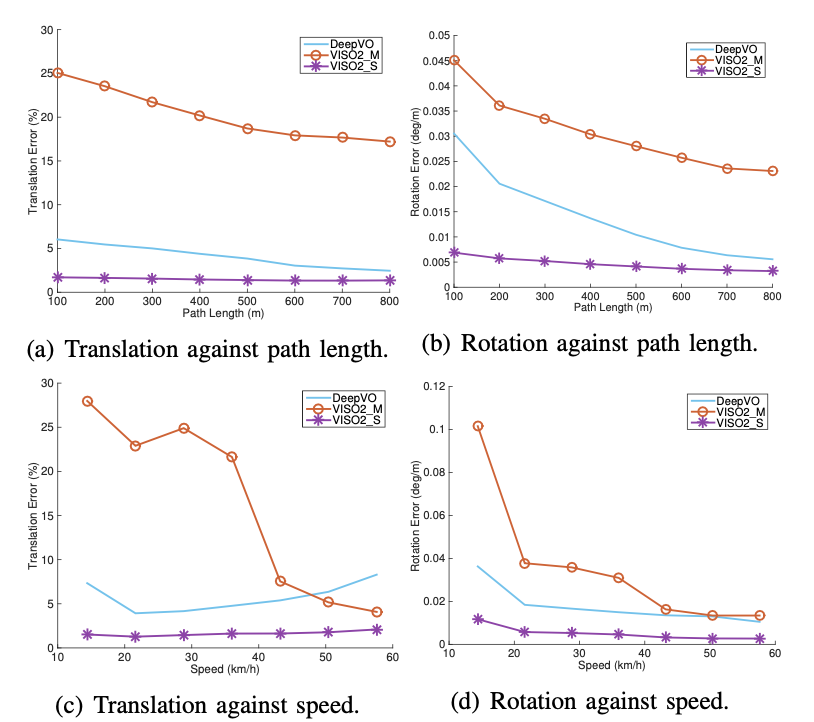
\includegraphics[width=0.65\columnwidth]{figuras/figura13.png}
        \caption{Average errors on translation and rotation against different path lengths and speeds for the Wang paper.}
        \label{fig:13}
    \end{figure}
    
    \begin{figure}[h]
        \centering
        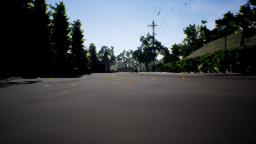
\includegraphics[width=0.65\columnwidth]{figuras/neig.png}
        \caption{Example of image obtained at the Neighbourhood scene from AirSim.}
        \label{fig:neig}
    \end{figure}
    
    \begin{figure}[h]
        \centering
        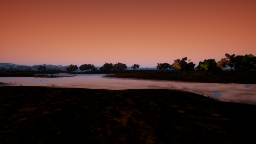
\includegraphics[width=0.65\columnwidth]{figuras/africa.png}
        \caption{Example of image obtained at the Africa scene from AirSim.}
        \label{fig:africa}
    \end{figure}
    
    \begin{figure}[h]
        \centering
        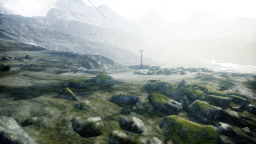
\includegraphics[width=0.65\columnwidth]{figuras/mountains.png}
        \caption{Example of image obtained at the LandscapeMountains scene from AirSim.}
        \label{fig:mountain}
    \end{figure}
    
    \begin{figure}[h]
        \centering
        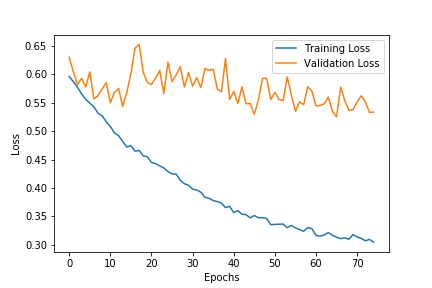
\includegraphics[width=0.65\columnwidth]{figuras/train_batch_dropout_90.png}
        \caption{Training losses without the weights of FlowNet.}
        \label{fig:train90}
    \end{figure}
    
    \begin{figure}[h]
        \centering
        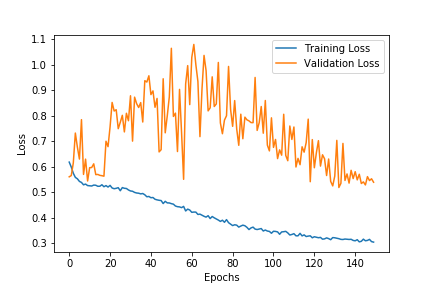
\includegraphics[width=0.65\columnwidth]{figuras/train_batch_dropout_150.png}
        \caption{Training losses with the weights of FlowNet.}
        \label{fig:train150}
    \end{figure}
    
    \begin{figure}[h]
        \centering
        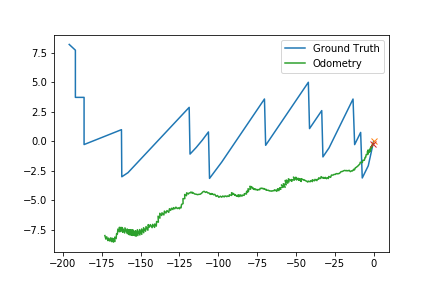
\includegraphics[width=0.65\columnwidth]{figuras/testeSeq2.png}
        \caption{Comparison between the ground truth position and the odometry provided by the system for the first test sequence.}
        \label{fig:seq2}
    \end{figure}
    
    \begin{figure}[h]
        \centering
        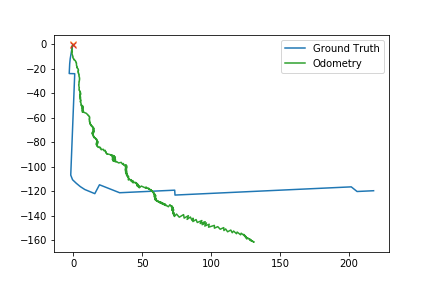
\includegraphics[width=0.65\columnwidth]{figuras/testeSeq4.png}
        \caption{Comparison between the ground truth position and the odometry provided by the system for the second test sequence.}
        \label{fig:seq4}
    \end{figure}
    
    \begin{figure}[h]
        \centering
        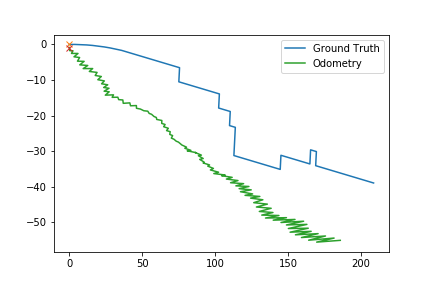
\includegraphics[width=0.65\columnwidth]{figuras/testeSeq5.png}
        \caption{Comparison between the ground truth position and the odometry provided by the system for the third test sequence.}
        \label{fig:seq5}
    \end{figure}